\documentclass[tikz,border=2pt]{standalone}
\usepackage{amsmath}
\usepackage{pgfplots}
\pgfplotsset{compat=1.18}
\usetikzlibrary{arrows.meta}

\begin{document}
% ||f||_∞ is the largest absolute value of f on X; ||f - g||_∞ is the widest vertical gap between
% two graphs, so it measures how far apart two functions are at their worst point.
% f(x) = 1.4 sin(pi x/3), g(x) = 0.5 sin(2 pi x/3) on [0, 2.8]: sup|f| = 1.4 at x = 1.5,
% the gap f - g is largest at x ~ 1.934 (value ~ 1.654).
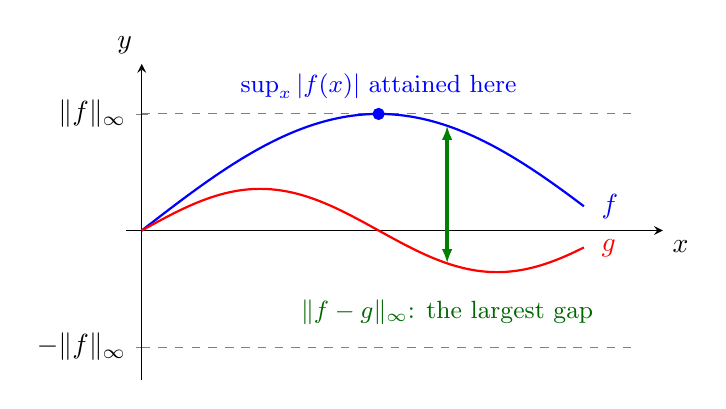
\begin{tikzpicture}
	\begin{axis}[
		axis lines=middle,
		xmin=-0.1, xmax=3.3,
		ymin=-1.8, ymax=2.0,
		xtick=\empty, ytick={1.4,-1.4}, yticklabels={$\|f\|_\infty$,$-\|f\|_\infty$},
		xlabel={$x$}, ylabel={$y$},
		xlabel style={below right}, ylabel style={above left},
		samples=200, smooth, clip=false,
		width=8.4cm, height=5.6cm
		]
		\addplot[gray, dashed, domain=0:3.1] {1.4};
		\addplot[gray, dashed, domain=0:3.1] {-1.4};
		\addplot[thick, blue, domain=0:2.8] {1.4*sin(deg(pi*x/3))};
		\addplot[thick, red, domain=0:2.8] {0.5*sin(deg(2*pi*x/3))};
		\addplot[only marks, mark=*, blue] coordinates {(1.5,1.4)};
		\draw[{Latex[length=1.8mm]}-{Latex[length=1.8mm]}, green!50!black, very thick] (axis cs:1.934,1.259) -- (axis cs:1.934,-0.395);
		\node[green!40!black, anchor=north, font=\small] at (axis cs:1.934,-0.72) {$\|f-g\|_\infty$: the largest gap};
		\node[blue, anchor=west] at (axis cs:2.85,0.29) {$f$};
		\node[red, anchor=west] at (axis cs:2.85,-0.21) {$g$};
		\node[blue, anchor=south, font=\small] at (axis cs:1.5,1.47) {$\sup_x|f(x)|$ attained here};
	\end{axis}
\end{tikzpicture}
\end{document}
